\documentclass[a4paper,beamer]{article}

\usepackage{graphicx}
\usepackage{tikz}
\usepackage{fix-cm}
\usepackage{chngpage}
\usepackage{fancyhdr}
\usepackage{rotating}
\usepackage[thinlines]{easytable}
\bibliographystyle{plain}
\usepackage[top=3cm,bottom=3cm,left=3.2cm,right=3.2cm,headsep=10pt,a4paper]{geometry} % Page margins
%\usepackage{fontspec}
%\setsansfont{Roboto}
%\renewcommand{\familydefault}{\sfdefault}

\pagestyle{fancy}
\fancyhf{}

\begin{document}
	\title{ System's Requirements Analysis and Design}
	\author{Group No: 10}
	\date{July 2017}

	% cover image
	\bgroup
		\tikz[overlay,remember picture]
		\node[opacity=1, at=(current page.center)] {
			
\includegraphics[height=\paperheight,width=\paperwidth]{img/cover}};
			
		\begin{adjustwidth}{-1cm}{-1.6cm}
			\textsf{\flushright\vfill\color{white}
				\fontsize{45}{60}\selectfont\textsf{Automated Minute\\ Tracker} \\[.8cm]
				\huge  System's Requirements Analysis and Design \\[.3cm]
				\huge Group No: 10 \\}
		\end{adjustwidth}
	\egroup
	%\maketitle
	\newpage
	
	% set header and footer
	\fancyhead[L]{System's Requirements Analysis and Design}
	\fancyhead[R]{Automated Minute Tracker}
	\fancyfoot[R]{\thepage \, \textbf\textbar \, \color{gray}  P A G E}
	\renewcommand{\footrulewidth}{0.1pt}
	
	% contents
	\tableofcontents
	\newpage
	
	\section{Introduction}
	
	\subsection{About the Client}
	
	University of Colombo School of Computing holds a monthly general meeting to  discuss about the student matters , operational details and other matters of the board. Every meeting has its agenda and the minute which contains the details discussed in the previous minute.\\
	
	Each minute matter is discussed twice and after  approval of any minute matter in its 2nd hearing  is been sent to the  Board of study (BOS), Academic Syndicate, Board of Management(BOM) and finally to the Senate. Every matter does not reach the senate. The priority level(until which level a minute matter should be reached) is been decided by the IUD.Whenever a matter is being rejected, it is sent back to the IUD. Then the IUD tries to re discuss it  by making relevant changes to the matter. Some urgent matters are being fast tracked directly to the higher board expecting a quick response. This project  mainly focuses  on a minute tracking process for BOS/IUD (Board of Study/Internal Undergraduate Degree)of UCSC which helps to know what matters are approved and what are rejected, which level the matter is being discussed now etc. Creating this automated minute tracker  helps to maintain a very stable way of storing, manipulating and tracking  all the minutes of monthly general meetings.
	
	\subsection{Domain Description}
	This product will be offered as a web-based platform service.This  lets only a limited amount of members (staff members and limited number of students) to login so all the details  so that the minutes are well secured. The system sends email containing the information about the next meeting to all the staff members. The editing privileges are limited only to secretary and assistant registrar. The review privileges are limited only to the Head of IUD and Director. whenever a staff member needs to find out which stage the minute matter is situated (IUD, Academic Syndicate, Board of Banagement, Senate) the system indicates the stage of the minute matter.\newline
	
	All the results (approved/reject/hold on) of minute matters are visible to members so that every stage is aware of the result of the minute matter, either it is accepted or rejected. After every meeting the whole document is being saved in the database .Incase if any member wants to find  out a minute of a previous meeting, the system helps filtering the needed minute.
	Fast tracked minutes are saved in another format so  they can be identified easily.\newline
	
	\subsection{Current System}
	Currently all the minutes are stored physically as files .This has caused  storage problems and also cumbersome to search previous minutes. The minute documents also have the  tendency to get damaged over time. The main problem the staff suffers is it takes a lot of time when finding previous minutes and the status (approved/rejected/hold on) of the minute. So that the workload on staff members is high.
	
	\subsection{Objectives and Goals}
	\begin{itemize}
		\item To make efficient the tracking of previously generated minutes which was vainly time consuming due to the bulk physical documentation.
		\item To make staff member know easily  which level a minute matter is been discussed.
		\item To clarify the status of matters of previous minutes.
		\item To form an easily accessible portal for the relevant users to state their issues, complaints or matters.
		\item To reduce the workload of the staff members 
	\end{itemize}
	
	\subsection{Scope of the Project}
	\begin{itemize}
		\item The project would create an online system to insert matters into a database.
		\item The minute will be able to auto generated and sent to all the users.
		\item The system enables to track whether where the matter is now in the approval process and check whether it is approved or being on hold.
		\item It will provide a database to store minutes.
	\end{itemize}
	
	\subsection{Assumptions and Constraints}
	
	\subsubsection{Assumptions}
	\begin{itemize}
		\item Users should be familiarized with the way of using a web application.
		\item System is only prepared for the IUD but it also can be used to other stages with some modifications.
	\end{itemize}
	
	\subsubsection{Constraints}
	\textbf{Time and Security Constraints} \newline\newline
	This project should be completed within a period of one year. The team has made decisions to complete the half of the project by the end of the 7  months. It includes drawing necessary types of UML diagrams, designing of interfaces, completing 30\% of the project’s implementation.\newline\newline
	All data which would be inserted into the system should be given high security. The system should be developed in a safe manner, so that no external user who is not given access by the administrator could use or change important data stored in the system. Eg: SQL injection\newpage
	
	\section{Feasibility Study}
	Feasibility study is conducted to assess the practicality of the proposed system. Strengths, weaknesses of the proposed system would be discussed here. The impact the system could have on users of the system and the external people. Feasibility study would also be a measure to what extent people could take benefits over an existing system. Also the opportunities and threats in the external environment for the proposed system and the resources that would be used for development purposes would also be taken into consideration.\\\\
	By conducting a feasibility study the developers can have a proper understanding on to what extent the project could be made a success and if the proposed system could achieve the set objectives and goals effectively and efficiently.\\\\	
	In order to develop the web application as the solution to the existing system, feasibility study was conducted under the categories;
	
	\begin{itemize}
		\item Operational feasibility
		\item Cultural feasibility
		\item Economic feasibility
		\item Technical feasibility
		\item Schedule feasibility
		\item Legal feasibility
	\end{itemize}
	
	Due to the drawbacks of the existing system the client has expected a solution which would make the operations more effective and efficient. Hence considering all requirements stated by them we came up with the following solution.
	
	\subsection{Web Based System}
	\subsubsection{Operational Feasibility}
	The system proposed to IUD is a web based system. The system to be developed would not hinder the current work flow of the system as it is not connected with any other existing systems. It is an independent system which would be manipulated by the administrator of the system.(System administrators in accordance with the functional policies of the institute will do granting access levels.) Hence the system to be developed would not interrupt the existing system business environment of the organization in any means.\\\\
	Users will have to log in to the system using their user-names and passwords. Authentication of the user will limit the ability of unsecured entrance.\\\\
	Users could access the system and get the necessary information, based on the role of the user there are restrictions. Hence those who are given access to the system could perform their tasks based the tasks allocated to them.
	Proposed system meets the expected requirements of the client. It would make the manipulation of data easy and as the users would be enabled to access the system easily, requirements will be fulfilled.\\\\
	The system has many benefits that a user could gain.
	No additional troubles to go through complex installation processes. Will work through the usual web browser.\\\\
	No platform dependency. Any user can access the web site using their existing web browsers. The general users need not to have technical expertise to use the site.
	
	\subsubsection{Cultural Feasibility}
	Cultural feasibility would be a measure of how well the proposed system would adapt to the organizational environment. How the users will accept the new system how effectively it will work in the organizational environment.\\\\
	The system would be developed in a user friendly manner with attractive user interfaces (UI). Also the system would give easy access to important information which would be useful to perform day to day IUD minute related activities effectively and efficiently.
	It will reduce manual work and reduces the workload of users.
	System increases efficient functioning of other related organizational activities as well. Therefore it saves time.
	
	\subsubsection{Economical Feasibility}
	Economical feasibility is an assessment of the possible positive economic benefits that the organization could gain out of the proposed system. It includes the cost or benefits analysis. All software that would be used in the development process are open source and available free. No costly hardware devices would be used. All required tasks would be performed by the team members, hence outsourcing would not be necessary.
	
	\paragraph{\textbf{Cost Benefit Analysis}}
	\begin{itemize}
		\item Reduces manual work
		\item Very high levels of readily available information
		\item Very interactive user interface
		\item Facilitates users to access the information efficiently
		\item All data would be organized
	\end{itemize}
	
	\paragraph{\textbf{Costs}}
	\begin{itemize}
		\item Hardware cost -
		Not necessary to purchase new hardware. Existing resources and hardware which belongs to developers would be used.
		\item Software cost - 
		Free and open source software would be used for development purposes.
		\item Operational cost(to the client when using the site)-
		PCs and other technical equipment cost
		Internet access
		Software costs in development
	\end{itemize}
	
	\subsubsection{Technical Feasibility}

	Technologies that would be used in order to develop the system
	Currently there are plenty of resources available to develop a web based application and an android application
	\begin{itemize}
		\item Web development
		Client side scripting: HTML, javascript, AngularJS, CSS
		Server side scripting: PHP, Codeigniter
		\item Web servers : Apache
		\item  Database management systems : MySQL
	\end{itemize}

	\noindent\textbf{Is the proposed solution practical?}\newline
	All technologies mentioned above are matured enough to build a stable web application which will be recognized. Every single module that would be implemented in the system have been implemented previously in certain systems, hence development of this system is a possible task.\newline
	
	\noindent\textbf{Do we currently possess the necessary technology?}\newline
	All the technologies mentioned above are open source and available free. Hence possession of technology will not be an issue.\newline`
	
	\noindent\textbf{Do we have the expertise needed to develop the solution?}\newline
	All members are familiar with technologies which will be used in the development. And the members are willing to share the knowledge they possess with other members when necessary. All members will put their maximum effort in order to make this project a success.\newline
	
	\subsubsection{Schedule Feasibility}
	Schedule feasibility measures if it is a possible task to complete the project within a particular time frame.\newline
	The Gantt chart prepared shows the mandatory deadlines that all group members are expected to achieve. Tasks are allocated to each member based on the capacities considering all other external factors. \newline

	\vspace{1cm}
	\noindent\textbf{Gantt chart (2017/2018)}
	\begin{figure}[h]
		\begin{center}
			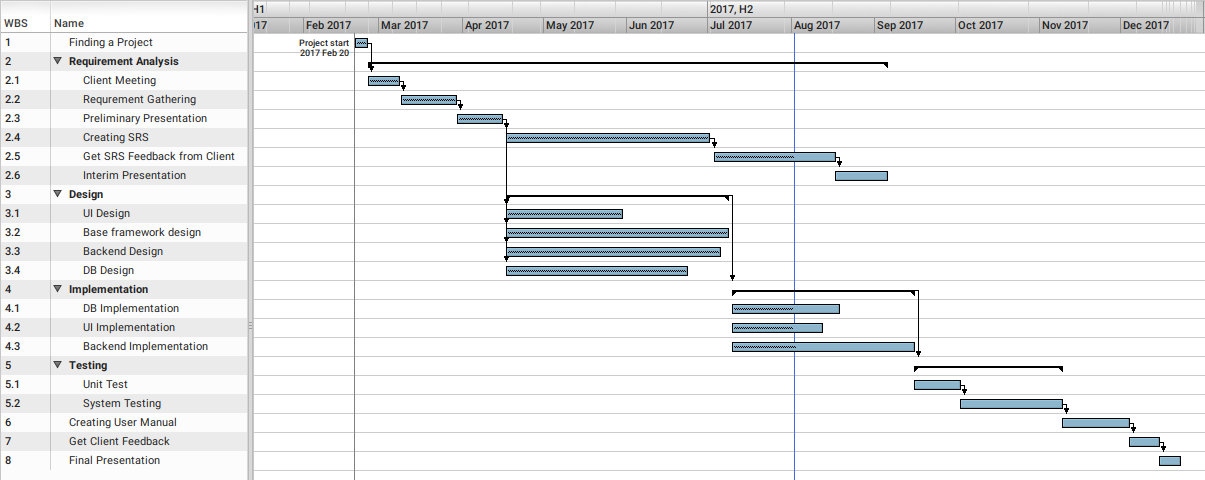
\includegraphics[width=6in,height=2.5in]{img/gantt}
		\end{center}
		\caption{The Gantt Chart}
		\label{fig:gantt}
	\end{figure}
	\newpage

	\subsubsection{Legal Feasibility}
	Determines whether the proposed system conflicts with the existing legal requirements. Legal feasibility verifies the legal validity of the proposed system.\newline
	\newline
	\textbf{Copyrights Issues}\newline
	We will be using free and open source technologies and tools for developing purposes. Hence there would be no violation of laws. We would not be using any articles or images from any other publications.\newline
	\newline
	\textbf{Government Constraints}\newline
	The proposed system will be implemented in a government organization. Hence it may be subjected to rules and regulations imposed.\newline
	All the information will be under the authority of the system administrator. Hence all the information is secured. Only the people who would be granted access by the administrator could access the system. Based on the role they would be performing privileges would be given.\newline
	
	\newpage
	
	\section{Requirements}
	
	\subsection{Stakeholders}
	There are four actors are involved with the system.\newline
	
	\begin{itemize}
	\item\textbf{Administrator} \\
		Person who is responsible for all the functions of the system. He is the person who could grant access to others to use the system under conditions.
	\item\textbf{Secretary, Assistant Registrar} \\
		Apart from the administrator, the secretary of IUD and assistance registrar is given authority to handle the system performing all operations.For example recommending matters, amending minute, generating minute.
	\item\textbf{Director}\\
		Auto generated minute will be produced to the director for different purposes 
	\item\textbf{Members,IUD}\\
		Members of IUD who submits memos to the online system, which are related to different matters.
	\end{itemize}
	
	\subsection{Use cases}
	
		\textbf{Use case narratives}\\
		%We need to have 15 use case narratives.\\

		% Start Tables
		\bgroup
			\def\arraystretch{2}% row height
		
			\begin{tabular}{|p{4cm}|p{8cm}|} \hline 
					\textbf{Use case ID} & \textbf{UC01}  \\ \hline
					Name & Login to the System \\ \hline 
					Description & Member login to the system \\ \hline 
					Primary actors & Member \\ \hline 
					Secondary actors & None \\ \hline 
					Pre Conditions & 1. Enter username. \\
												& 2. Enter password.\\ \hline 
					Main Flow & 1. Enter username \\
										& 2. Enter Password \\  
										& 3. The use case ends. \\ \hline
					Postconditions & None \\ \hline 
			\end{tabular} \\[.6cm]
			
			\begin{tabular}{|p{4cm}|p{8cm}|} \hline 
					\textbf{Use case ID} & \textbf{UC02}  \\ \hline
					Name & Check the status of a minute matter \\ \hline 
					Description & Member checks whether the minute matter is approved  , rejected or in ‘ hold on’ status \\ \hline 
					Primary actors & Member \\ \hline 
					Secondary actors & None \\ \hline 
					Pre Conditions & None \\ \hline 
					Main Flow & 1. Log into the system. \\
										&	2.1. Search the matter in the selected criteria. \\
										&	2.1.1. View the matter \& check the matter status (approved , rejected, hold on) \\
										&	2.1.2. Searched matter does not exist.\\ 
										&	2.2. View existing matter \& check the status.  \\
										&	3. The use case ends.\\ \hline		
					Postconditions & None \\ \hline 
			\end{tabular} \\[.6cm]
			
			\begin{tabular}{|p{4cm}|p{8cm}|} \hline 
					\textbf{Use case ID} & \textbf{UC03}  \\ \hline
					Name & Check the stage where the minute matter is discussed. \\ \hline 
					Description & Member checks in which level the minute matter is being discussed (IUD,Academic Syndicate,Board of management or senate) \\ \hline 
					Primary actors & Member \\ \hline 
					Secondary actors & None \\ \hline 
					Pre Conditions & None \\ \hline
					Main Flow & 1. Log into the system. \\
										& 2.1 Search the matter in the selected criteria.\\
										& 2.1.1 View the matter \& check the level of the matter where it is being discussed. \\
										& 2.1.2 Searched matter does not exist. \\
										& 2.2 View existing matter \& check the level of the matter\\
										& 3. The use case ends.\\ \hline
					Postconditions & None \\ \hline 
			\end{tabular} \\[.6cm]
				
			\begin{tabular}{|p{4cm}|p{8cm}|} \hline 
					\textbf{Use case ID} & \textbf{UC04}  \\ \hline
					Name & Search previous minute matters.\\ \hline 
					Description & Member checks  matters of previous minutes.\\ \hline 
					Primary actors & Member \\ \hline 
					Secondary actors & None \\ \hline 
					Pre Conditions & None \\ \hline
					Main Flow & 1. Log into the system.\\
							& 2. Search the matter in the selected criteria.\\ 
							& 2.1  Search using a keyword \\
							& 2.2  Search  using minute ID\\
							& 2.3  Searched matter does not exist\\
							& 3. The use case ends.\\ \hline
					Postconditions & None \\ \hline 
			\end{tabular} \\[.6cm]
			
			\begin{tabular}{|p{4cm}|p{8cm}|} \hline 
					\textbf{Use case ID} & \textbf{UC05}  \\ \hline
					Name & Submit memo \\ \hline 
					Description & Submitting  memos (a new matter )to the system \\ \hline 
					Primary actors & Member \\ \hline 
					Secondary actors & None \\ \hline 
					Pre Conditions & None \\ \hline
					Main Flow & 1. Log into the system.\\
										& 2. Enter the new memo. \\
										& 3. Save the entered memo.\\
										& 4. The use case ends.\\ \hline
					Postconditions & None \\ \hline 
			\end{tabular} \\[.6cm]
			
			\begin{tabular}{|p{4cm}|p{8cm}|} \hline 
					\textbf{Use case ID} & \textbf{UC06}  \\ \hline
					Name & Discuss any other business II \\ \hline 
					Description & Only a staff member can view any other business II \\ \hline 
					Primary actors & Staff Member \\ \hline 
					Secondary actors & None \\ \hline 
					Pre Conditions & None \\ \hline
					Main Flow & 1. Log into the system.\\
										& 2. View any other business II \\
										& 3. The use case ends.\\ \hline
					Postconditions & None \\ \hline 
			\end{tabular} \\[.6cm]
			
			\begin{tabular}{|p{4cm}|p{8cm}|} \hline 
					\textbf{Use case ID} & \textbf{UC07}  \\ \hline
					Name & Review minutes \\ \hline 
					Description & Director review the minute document \\ \hline 
					Primary actors & Director \\ \hline 
					Secondary actors & None \\ \hline 
					Pre Conditions & None \\ \hline
					Main Flow & 1. Log into the system.\\
										& 2. View the minute document before the  document is emailed. \\
										& 3. Mark changes that should be done.\\
										& 4. Save the edited changes \\
										& 5.End use case \\ \hline
					Postconditions & None \\ \hline 
			\end{tabular} \\[.6cm]
			
			\begin{tabular}{|p{4cm}|p{8cm}|} \hline 
					\textbf{Use case ID} & \textbf{UC08}  \\ \hline
					Name & Administrating the System \\ \hline 
					Description & The whole system is administered by The Secretary \\ \hline 
					Primary actors & Secretary \\ \hline 
					Secondary actors & None \\ \hline 
					Pre Conditions & None \\ \hline
					Main Flow &	1. Log into the system.\\
										& 2. Administrative works of the System\\
										& 3. The use case ends.\\ \hline
					Postconditions & None \\ \hline 
			\end{tabular} \\[.6cm]
			
			\begin{tabular}{|p{4cm}|p{8cm}|} \hline 
					\textbf{Use case ID} & \textbf{UC09}  \\ \hline
					Name & Generate/Edit the minute document. \\ \hline 
					Description & Secretary Generate/Edit the minute document \\ \hline 
					Primary actors & Secretary \\ \hline 
					Secondary actors & None \\ \hline 
					Pre Conditions & None \\ \hline
					Main Flow &	1. Log into the system.\\
										& 2.1 Generate the minute document\\
										& 2.1.1 add memos\\
										& 2.1.2 add previously discussed matters for their 2nd hearing \\
										& 2.1.3 add matters for any other business II\\
										& 2.2 Edit the minute document \\
										& 2.2.1 Remove unwanted matters\\
										& 2.2.2 Amendment of matters\\
										& 3. Save the edited/generated  matters.\\
										& 4. The use case ends.\\ \hline
					Postconditions & None \\ \hline 
			\end{tabular} \\[.6cm]
			
			\begin{tabular}{|p{4cm}|p{8cm}|} \hline 
					\textbf{Use case ID} & \textbf{UC10}  \\ \hline
					Name & Recommend matters after first hearing \\ \hline 
					Description & Secretary recommend new matters after the first hearing \\ \hline 
					Primary actors & Secretary \\ \hline 
					Secondary actors & None \\ \hline 
					Pre Conditions & None \\ \hline
					Main Flow & 1. Log into the system.\\
										& 2. Recommend new matters as memo cards.\\
										& 3. Save the edited changes \\
										& 4. The use case ends.\\ \hline
					Postconditions & None \\ \hline 
			\end{tabular} \\[.6cm]
			
			\begin{tabular}{|p{4cm}|p{8cm}|} \hline 
					\textbf{Use case ID} & \textbf{UC11}  \\ \hline
					Name & Extract matters and submit to the academic syndicate \\ \hline 
					Description & Secretary Extract the matters which are approved , amended for further discussions or fast tracked matters and submit them to the academic syndicate \\ \hline 
					Primary actors & Secretary \\ \hline 
					Secondary actors & None \\ \hline 
					Pre Conditions & None \\ \hline
					Main Flow & 1. Log into the system.\\
							& 2.1. Select all approved matters\\
							& 2.2. Select all matters to be fast tracked\\
							& 2.3. Select all the matters that are amended for further discussions. \\
							& 3. Save them separately\\
							& 4. Edit if needed\\
							& 5. Save all the changes\\
							& 6. Submit to the academic syndicate\\
							& 4. The use case ends.\\ \hline
					Postconditions & None \\ \hline 
			\end{tabular} \\[.6cm]
		
	\egroup
	\newpage      
	
	\subsubsection{Use case Diagram}
	
	\begin{figure}[h]
		\begin{center}
			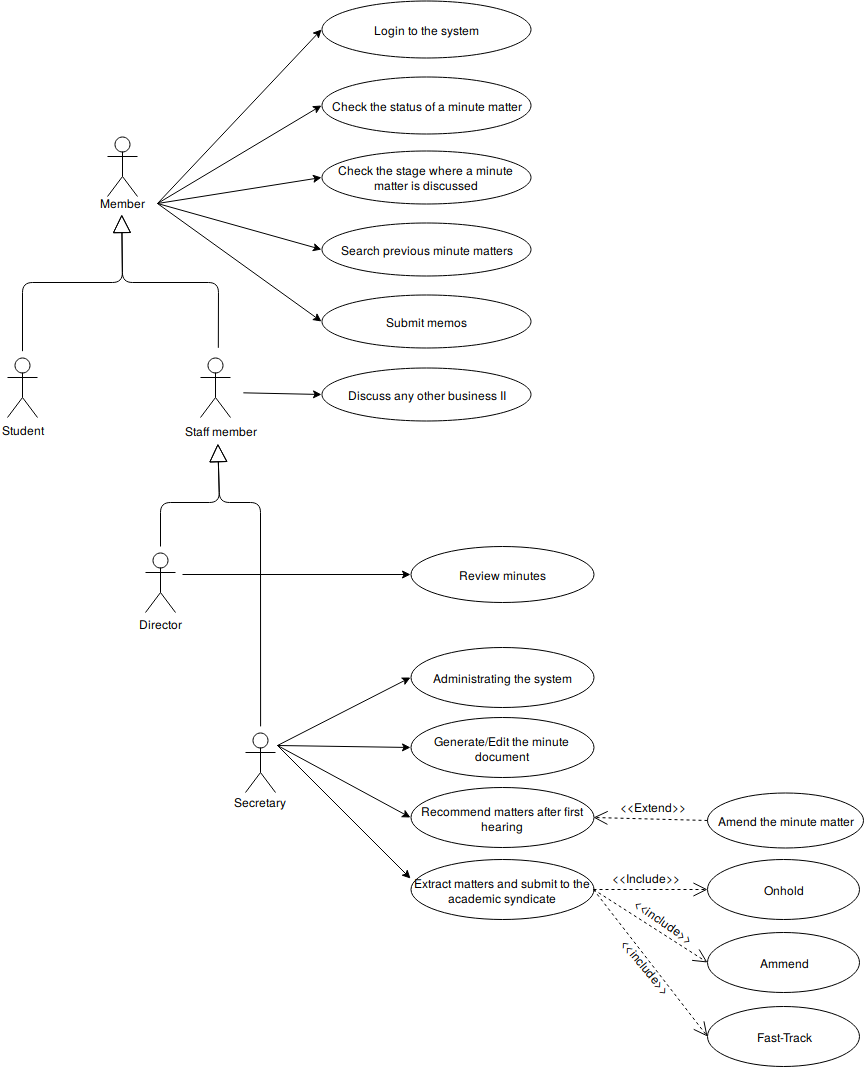
\includegraphics[width=6in,height=6in]{img/use-case-diagram}
		\end{center}
		\caption{The Use Case Diagram}
		\label{fig:usecase}
	\end{figure}
	\newpage        
	
	\subsection{Functional Requirements}
	\begin{enumerate}
		\item Login \newline
		Different users can access the system. Each user will have a role which defines the set of tasks which he/she can do. They are bound to certain conditions (based on their role) Administrator, Secretary,Staff member and Students can access the system. Privileges limit based on the actor. Example: Administrator can authorize access for a student to the System. But staff member can’t authorize access for the students.
		
		\item Adding User \newline
		Administrator can add users to the system and grant access to certain operations in the system.
		
		\item Privileged Accessibility \newline
		Every user is within a certain privilege criteria. For an example when the Administrator adds a student, he/she is not given the accessibility to reach out for the Any Other Business II category.
		
		\item Entry of Memos \newline
		A Digital portal is provided for the users to forward the relevant memos.
		
		\item Amending of memos \newline
		The Secretary is given the privilege to amend any memo after being decided to amend by the Board.
		
		\item Manipulation of memo proceedings \newline
		The Secretary has the option to recommend,hold or reject a memo.
		
		\item Auto Generation of minutes \newline
		The minute relevant to the most recent BOS/IUD meeting would be auto generated monthly. 
		
		\item Storing of Previous Minutes \newline The previously auto generated minutes are stored in a database to be checked if necessary in future.
		
		\item Tracking the minute \newline
		The generated minute could be tracked,which means that the user would be able to be acknowledged of the fact that what sort of a feedback has it been received by the higher levels and so on.
		
		\item Reviewing the minute \newline
		The Director should be able to review the auto-generated minute before it being released.
		
		\item Searching \newline
		The users can search for a certain matter within a previously generated minute via an ID or a Keyword.
		
	\end{enumerate}
	
	\newpage 
	
	\subsection{Non-Functional Requirements}
	\textbf{Performance}\\
	The system must be quick to respond to an action by a user. Retrieving information should be fast and users should be able to search queries fast. (Evaluated using response time) \newline
	\newline
	\textbf{Usability}\\
	The system should be usable by all the users (Administrator, Manager, Depot and General public) with minimal training. Interfaces must direct with a description briefing the usage of it.\newline
	\newline
	\textbf{Security}\\
	The main non-functional requirement of our system security. System must be capable of preventing SQL injunctions. Sensitive data must be properly encrypted. System components must be restricted and be accessed only if the user is privileged.\newline
	\newline
	\textbf{Accuracy}\\
	System must contain accurate data and produce accurate outputs after processing data.\\
	\newline
	\textbf{Maintainability}\\
	System components must be easy to modify, to correct faults and to adapt when new requirements are observed. System must contain separate storage for testing with real data before changed components active for the system’s use.\newline
	
	\newpage

	\section{System's Architecture}
	
	\subsection{Components and their Responsibilities}
	\begin{itemize}
		\item Login \& authentication - Validates the credentials of the user
		\item UAAPI - Assign access privileges and roles to the user.
		\item Control panel - Generating the system log.
		\item User management interface - Add/Edit Users.
		\item Restricted viewer - Generate details available for the normal user
		\item Data requesting and inserting layer - Validates whether the data is in correct format.
		\item Data access layer - Check user privileges
		\item Security layer - Establishing security measures
	\end{itemize}
	
	\subsection{Component Interactions}

	\begin{figure}[h!]
		\begin{center}
			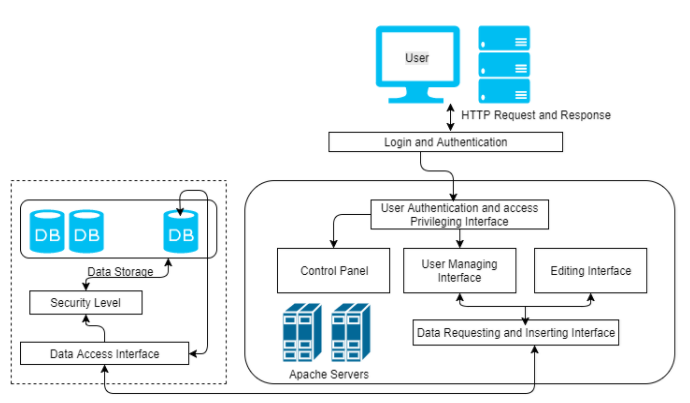
\includegraphics[width=6in,height=3in]{img/component-diagram}
		\end{center}
		\caption{The Component Diagram}
		\label{fig:component}
	\end{figure}
	\vspace{2cm}
	
	\newpage
	\begin{figure}[h]
		\begin{center}
			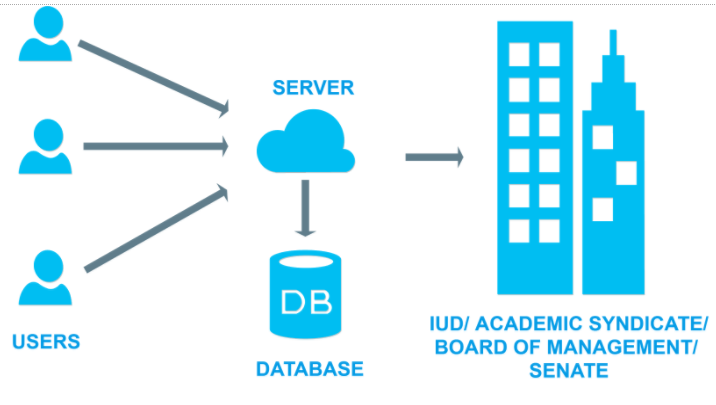
\includegraphics[width=5in,height=3in]{img/higher-level-architecture}
		\end{center}
		\caption{The Higher level Architecture}
		\label{fig:architecture}
	\end{figure}
	
	\newpage
	
	\section{System's Design}
	
	\subsection{Class Diagrams}
		\vspace{1cm}
		\begin{figure}[h!]
			\begin{center}
			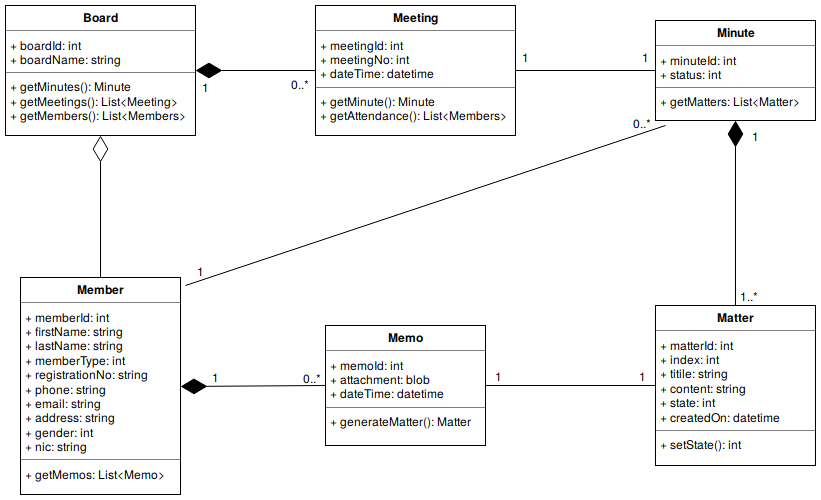
\includegraphics[width=6in,height=4in]{img/class-diagram}
			\end{center}
			\caption{Class Diagram}
			\label{fig:class-diagram}
		\end{figure}
		\newpage
	
	\subsection{Sequence Diagrams}
		\textbf{Log in}\newline
			
		\begin{figure}[h!]
			\begin{center}
			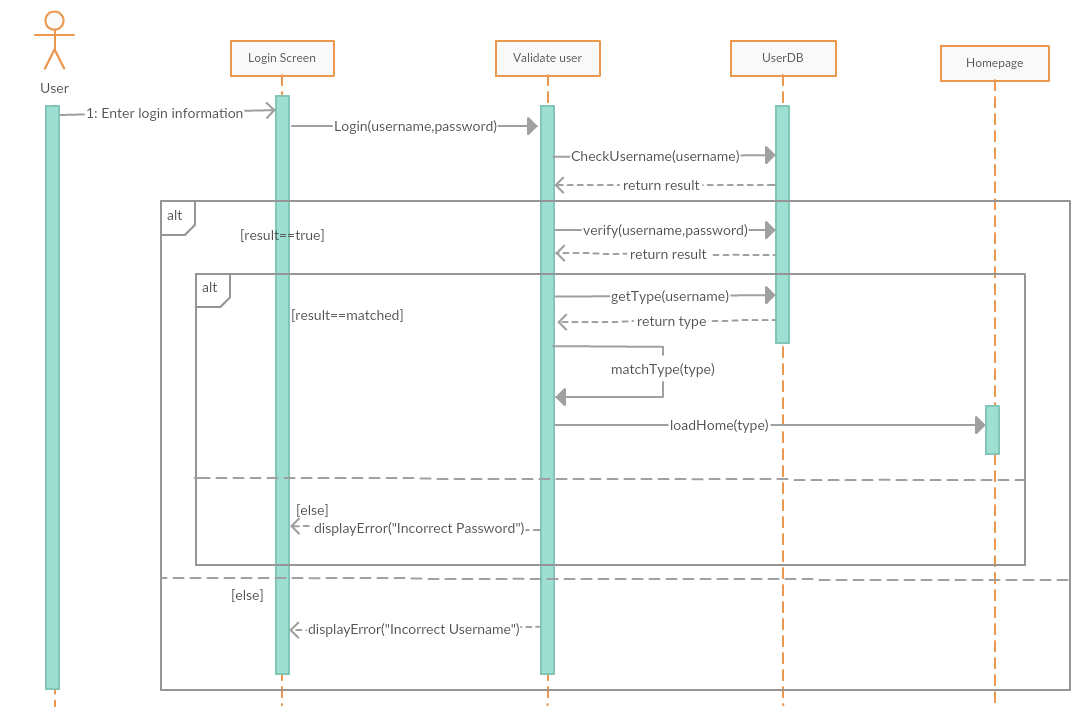
\includegraphics[width=6in,height=4in]{img/seq-login}
			\end{center}
			\caption{Log In}
			\label{fig:Log In}
		\end{figure}

		 Users who are signed up with system can log into the system by entering their username and password.First there username is verified by the database and then the password is matched with the username.\\
		 
		Then, system will determine to which type (student, lecturer, etc.) the user belongs to, using the username.Then  the user is provided with a suitable view of home screen according to their type.\newline

		\newpage
		
		\textbf{Search Matter}\newline
		\begin{figure}[h!]
			\begin{center}
			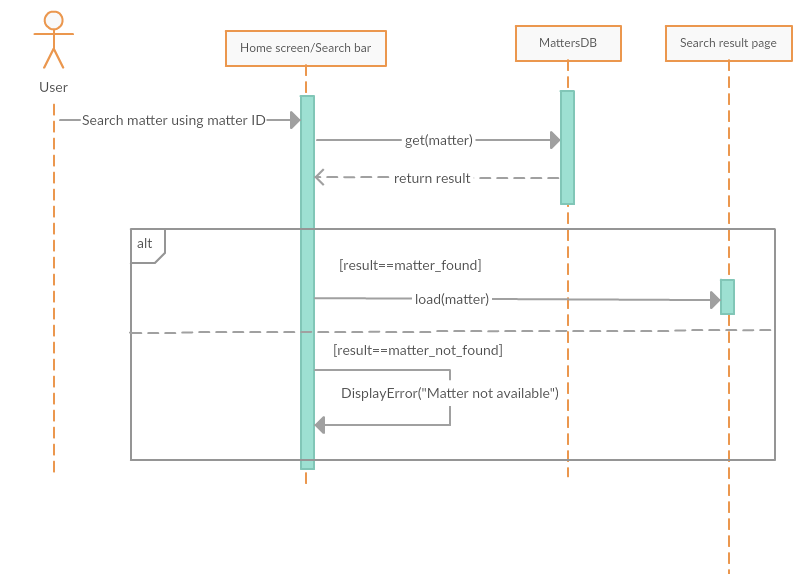
\includegraphics[width=6in,height=4in]{img/seq-search-matter}
			\end{center}
			\caption{Search Matter}
			\label{fig:search-matter}
		\end{figure}
		        
		Each matter stored in the matter database are assigned with an unique ID (primary key).Users can use these matter IDs to search matters.\newline
		
		Within the web application we can find a search bar in top of every window. By entering matter IDs on these search bar users can get data (eg: statuses of the matters) of the matters on a search result page. \newline
		
		A matter will be displayed on the search result page if the entered ID is correct  unless it have been deleted from the database nor the database is not updated with the minute at the point.\newline
		\newpage
		
		\textbf{Edit Matter}\newline
		\begin{figure}[h!]
			\begin{center}
			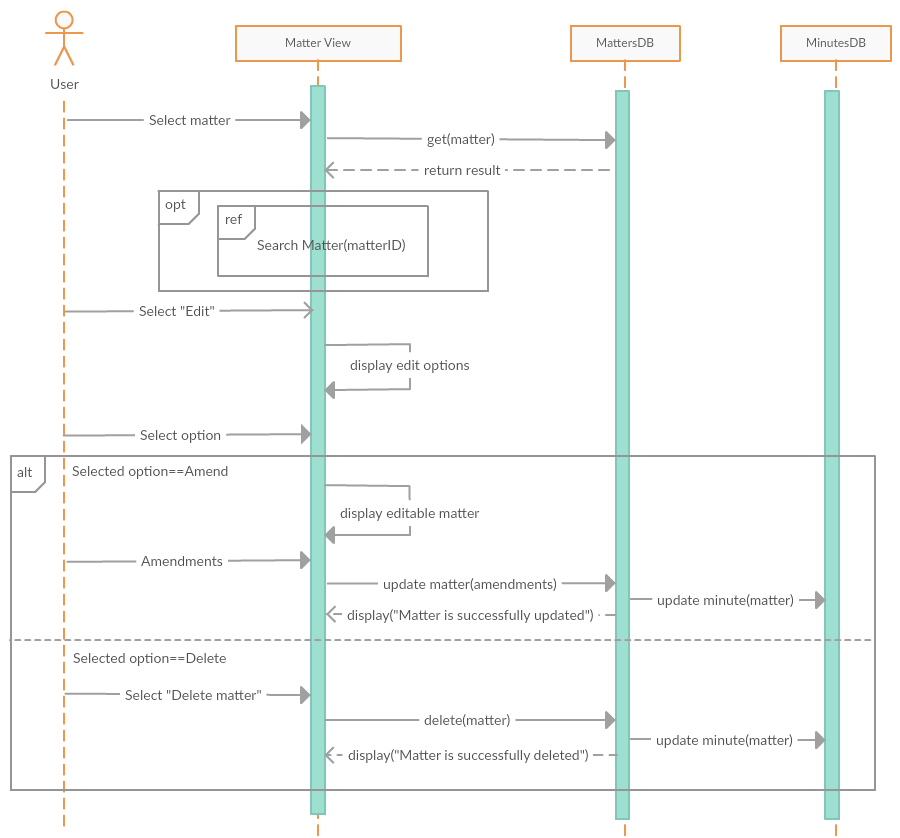
\includegraphics[width=6in,height=5in]{img/seq-edit-matter}
			\end{center}
			\caption{Edit Matter}
			\label{fig:edit-matter}
		\end{figure}
		        
		When its comes to editing a matter, users can amend matters or delete matters from the database.Users can select a matter to be edited using the matter view window or by searching for matter by its ID.
		
		When amending the users get the chance to edit the content of a matter.

		When a minute is edited(amended or deleted) first the matters database is updated and then if the relevant edited matter is included in a minute then with the updated matter, minute is also get updated.\newline
		\newpage
		
		\textbf{Review/Track Matter}\newline
		\begin{figure}[h!]
			\begin{center}
			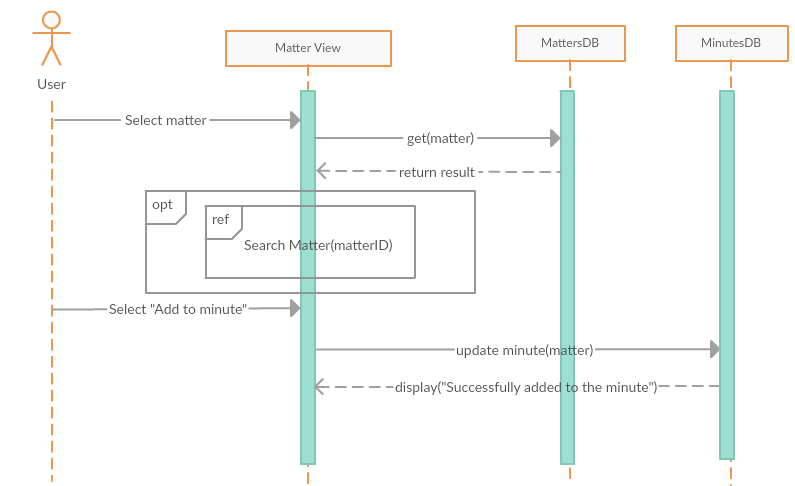
\includegraphics[width=6in,height=4in]{img/seq-review-matter}
			\end{center}
			\caption{Review-Matter}
			\label{fig:review-matter}
		\end{figure}
		        
		Users have to select a matter before reviewing, for that they can either search for it using matter ID or select a matter in the matters view window. By selecting a matter the user can get all the necessary data of a matter stored in the matter database.Users can check wheather the minute is beign rejected or approved and they can get the details about at which level, currently the matter is beign dicussed.By using these data about the matter, users can review the matter and decide wheather the matter is beign finalised, and if the matter is suitable to be added to the minute they can update the minute by adding the matter into the minute.
		
		\newpage
	
	\subsection{User Interface Flow Diagram}
		\vspace{2cm}
		\begin{figure}[h!]
			\begin{center}
			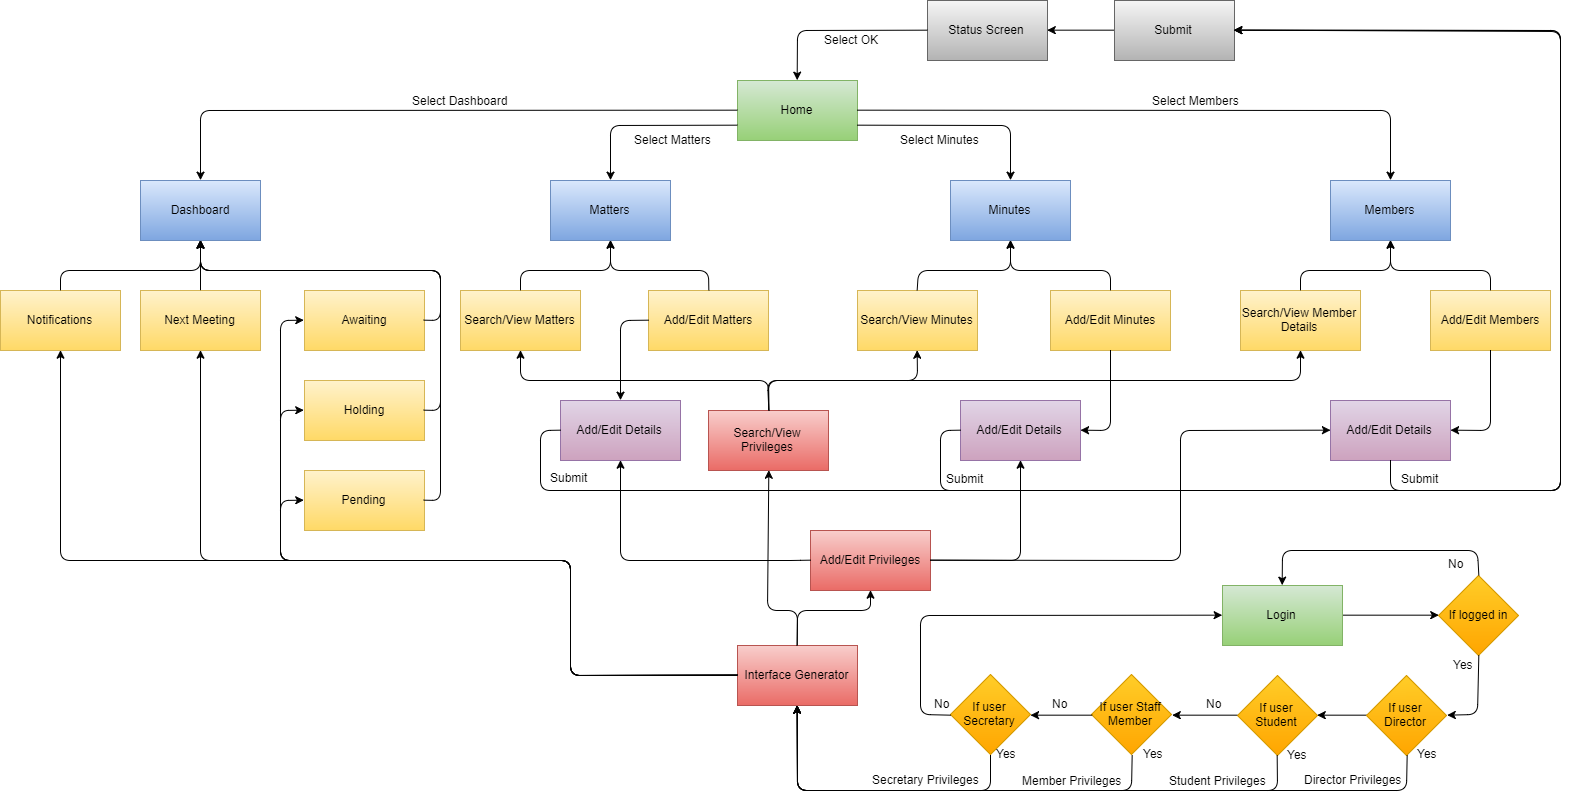
\includegraphics[width=6in,height=3in]{img/user-interface-flow}
			\end{center}
			\caption{User Interface Flow Diagram}
			\label{fig:user-interface-flow}
		\end{figure}
		\newpage
		
		\vspace{1cm}
		\begin{figure}[h!]
			\begin{center}
			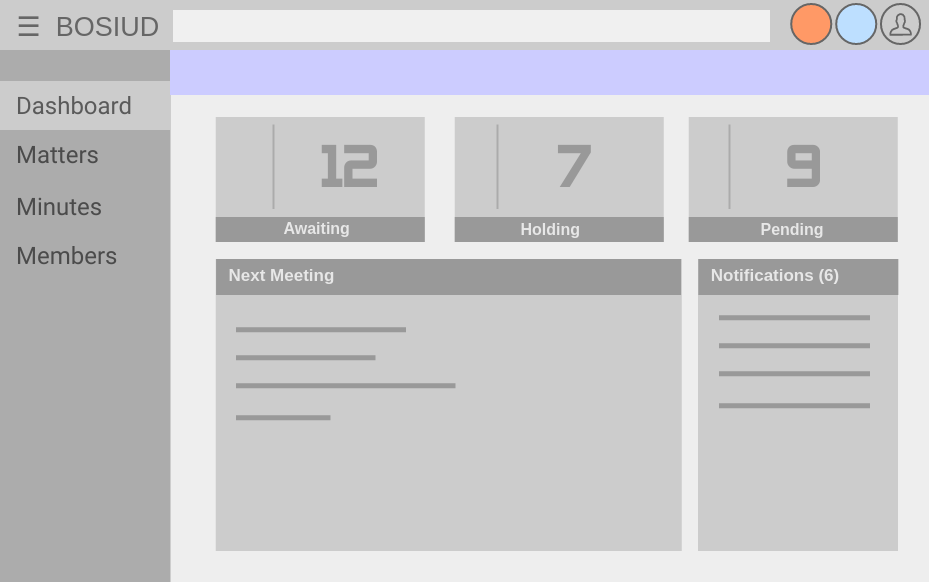
\includegraphics[width=5in,height=3in]{img/ui-dashboard}
			\end{center}
			\caption{Dashboard View}
			\label{fig:ui-dashboard}
		\end{figure}

		\begin{figure}[h!]
			\begin{center}
			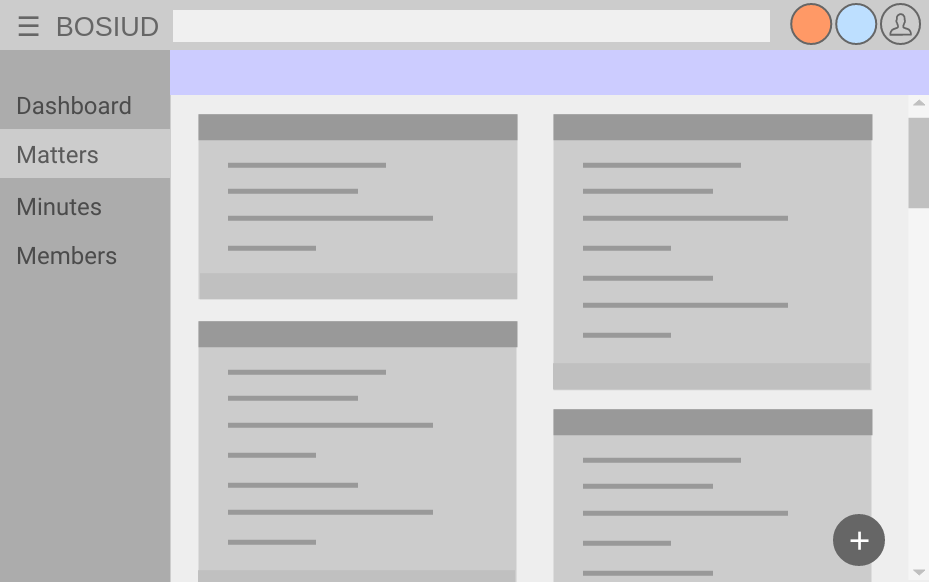
\includegraphics[width=5in,height=3in]{img/ui-matters}
			\end{center}
			\caption{Matters View}
			\label{fig:ui-matters}
		\end{figure}

		\begin{figure}[h!]
			\begin{center}
			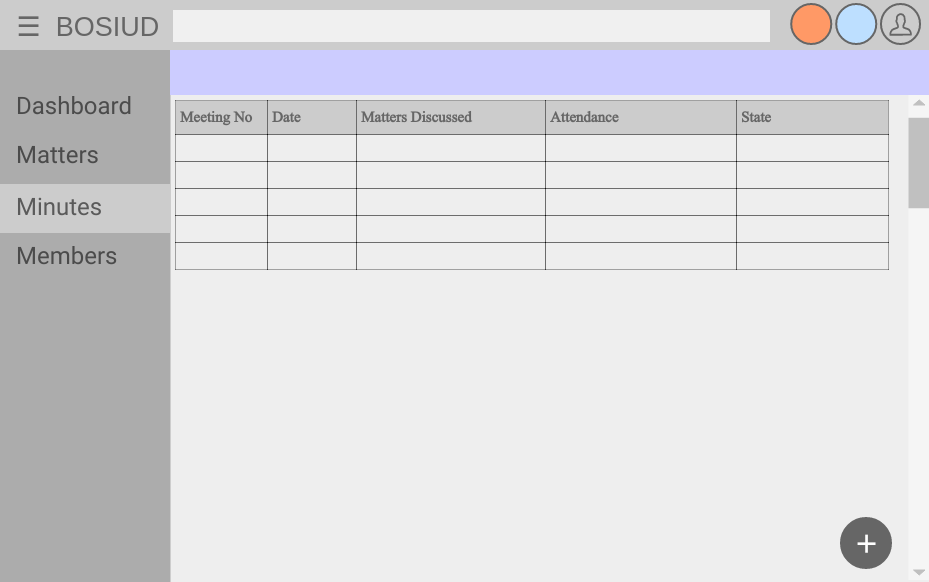
\includegraphics[width=5in,height=3in]{img/ui-minutes}
			\end{center}
			\caption{Minutes View}
			\label{fig:ui-minutes}
		\end{figure}
		
		\begin{figure}[h!]
			\begin{center}
			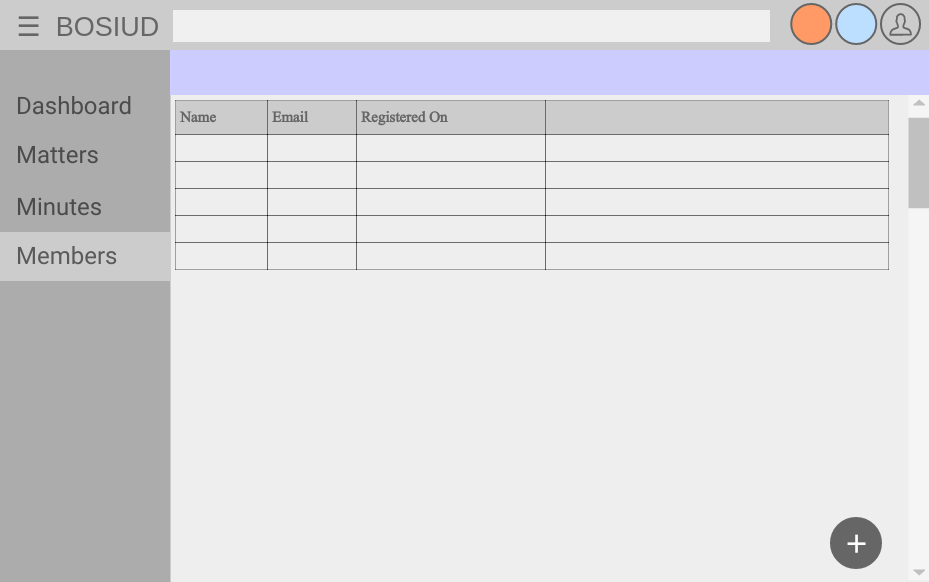
\includegraphics[width=5in,height=3in]{img/ui-members}
			\end{center}
			\caption{Members View}
			\label{fig:ui-members}
		\end{figure}
		
		\clearpage
		\newpage

	\subsection{Entity Relationship Diagram}
		\vspace{2cm}
		\begin{figure}[h]
			\begin{center}
				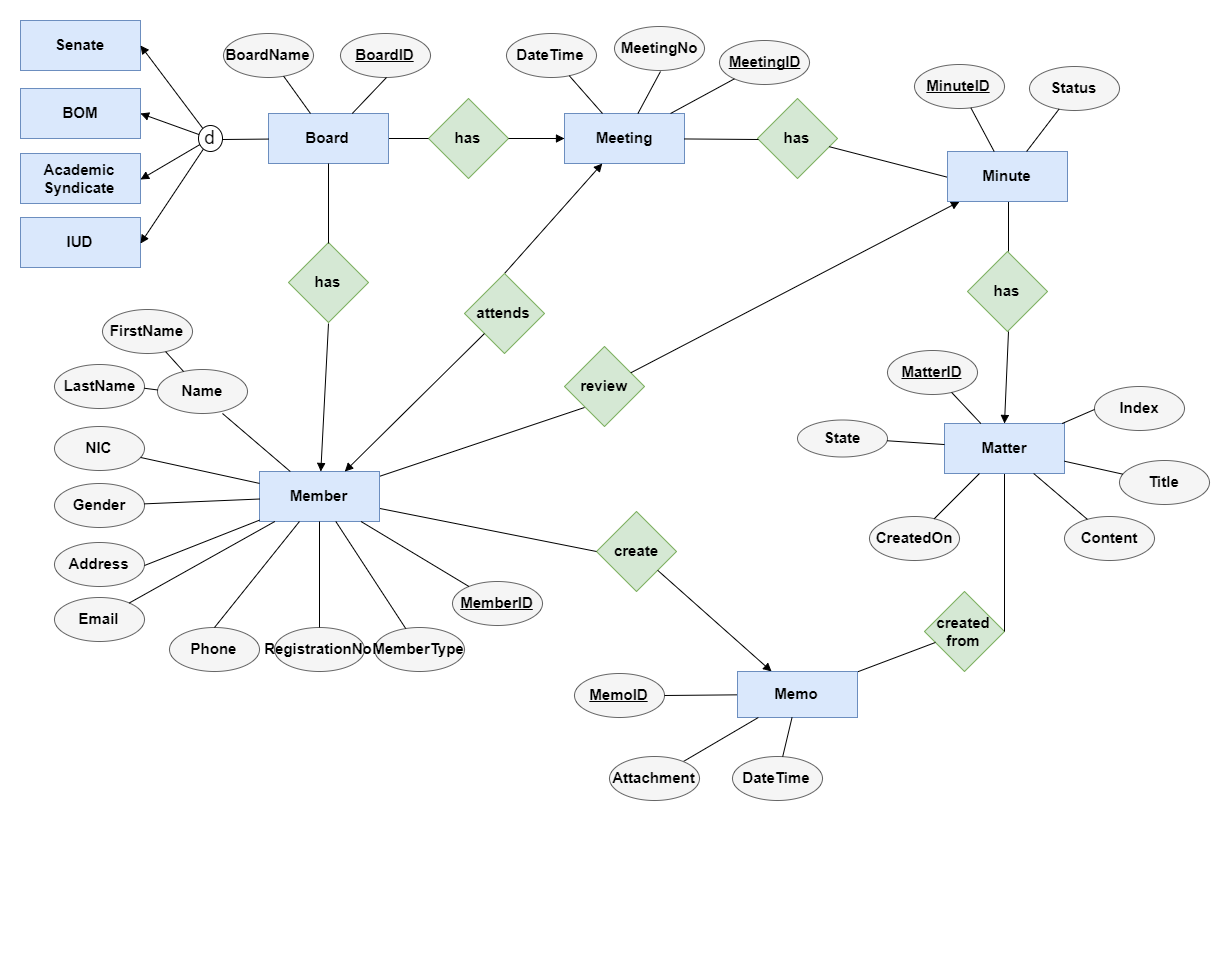
\includegraphics[width=6in,height=5in]{img/entity-relationship-diagram}
			\end{center}
			\caption{The Entity Relationship Diagram}
			\label{fig:ERD}
		\end{figure}
		\newpage  
	
		%Group details
		\textbf{Group Details}\\
		\vspace{1cm}\\	
				\bgroup
					\def\arraystretch{2}% row height
					\begin{tabular}{|p{.5cm}|p{5cm}|p{4cm}|p{3cm}|} \hline 
					  & \textbf{Full Name}  & \textbf{Registration Number} & \textbf{Index No } \\ \hline
					1) & D.M.S Dissanayake	 & 2015/CS/038 & 15000389\\ \hline
					2) & H. Chamika  P.  Hewainna & 2015/IS/028 & 15020282\\ \hline
					3) & S.D.P Devotta & 2015/CS/031 & 15000311\\ \hline
					4) & Samadhi S.P Abeywickrama & 2015/CS/004 & 15000044\\ \hline
					5) & B.C.P.S.K. Peiris	 & 2015/CS/094 & 15000941\\ \hline
					6) & G.Y.A.C Sarathchandra & 2015/IS/069 & 15020691\\ \hline
					\end{tabular} \\[.6cm]
				\egroup
	
\end{document}
